% SC4012 --- Chapter 8: Secure Development Lifecycle (0->100 ground-up)
\chapter{Secure Development: SDL, CVSS and Incident Response}
\label{ch:secure-dev}

\begin{quote}
\emph{``Security is a lifecycle, not a feature.''} --- From the first requirement to the post-mortem after a breach, every phase has a security job. The SDL makes it explicit, CVSS makes it comparable, and response makes it survivable.
\end{quote}

\noindent\fbox{\parbox{\dimexpr\linewidth-2\fboxsep-2\fboxrule}{%
\textbf{From zero: how secure software is built.} We assume no process background. We walk the lifecycle phase by phase (requirements $\to$ design $\to$ code $\to$ test $\to$ deploy $\to$ respond), define CVSS scoring, and practice incident response as a rehearsed playbook.}}
\vspace{0.4em}

\section*{Learning Outcomes}
After this chapter you will be able to:
\begin{enumerate}[label=(L\arabic*)]
    \item map SDL activities to each development phase and argue their value;
    \item run a lightweight threat model in a design review (DFD + STRIDE);
    \item score a vulnerability with CVSS v3.1 base metrics and interpret severity;
    \item describe incident response phases (prepare, detect, contain, eradicate, recover, lessons);
    \item write a security requirement and a post-mortem that prevent recurrence.
\end{enumerate}

% ============================================================
\section{The Secure Development Lifecycle (SDL)}
\label{sec:sdl}
Intuition: fixing a bug in requirements costs $1\times$; fixing it after release costs $100\times$ (IBM/NIST data). The SDL (Microsoft, 2004) adds security activities to each phase so bugs are caught at the cheapest point.

\begin{figure}[h]\centering
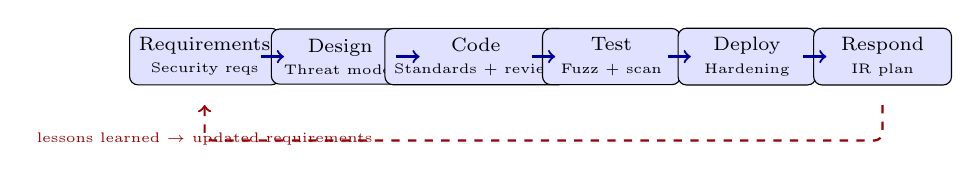
\begin{tikzpicture}[scale=0.82,every node/.style={font=\scriptsize}]
  \foreach \i/\lab/\act in {0/Requirements/Security reqs,%
    2.1/Design/Threat model,%
    4.2/Code/Standards + review,%
    6.3/Test/Fuzz + scan,%
    8.4/Deploy/Hardening,%
    10.5/Respond/IR plan} {
    \node[draw,fill=blue!12,rounded corners=3pt,minimum width=1.75cm,minimum height=0.7cm,align=center] at (\i,1.2) {\lab\\\tiny \act};
    \ifdim \i pt > 0pt \draw[->,thick,blue!60!black] (\i-1.23,1.2) -- (\i-0.87,1.2); \fi
  }
  \draw[->,thick,red!60!black,dashed,rounded corners=3pt] (10.5,0.45) -- (10.5,-0.1) -- (0,-0.1) -- (0,0.45) node[midway,below,font=\tiny] {lessons learned $\to$ updated requirements};
\end{tikzpicture}
\caption{SDL as a loop. Each phase has a security activity; the post-mortem feeds back into requirements. Skipping early phases shifts cost to the most expensive right-hand side.}
\label{fig:sdl-loop}
\end{figure}

Phase activities (lightweight version):
\begin{description}[leftmargin=1.2em,itemsep=0.30em]
    \item[Requirements] State security goals (CIA per asset), compliance needs, and abuse cases. Example: ``The system shall enforce that user A cannot read user B's data under any API call.''
    \item[Design] DFD + STRIDE (Ch.~1), pick crypto/sandbox primitives, write down trust boundaries.
    \item[Implementation] Secure coding standards (Ch.~2--4), safe defaults, code review with checklist, SAST (taint) in CI.
    \item[Verification] Fuzzing + sanitizers (Ch.~5), DAST/ZAP, and verification (Ch.~6) for critical components.
    \item[Release] Hardening (ASLR, W$\oplus$X, canaries, CSP, HSTS), secrets management, least privilege deploy.
    \item[Response] Monitor, detect, respond, and learn (see \S\ref{sec:ir}).
\end{description}

\begin{example}[Security requirement]
Bad: ``The app shall be secure.'' Good: ``The export endpoint shall return only rows where \texttt{tenant\_id = caller.tenant\_id}, enforced at the query layer, verified by a taint test that fails if a tenant-unqualified query reaches the DB sink.'' A good requirement is testable and maps to a sink that CI can check.

\end{example}

\begin{example}[Threat model in 30 minutes]
A new ``export CSV'' feature: draw the DFD delta (DB $\to$ service $\to$ HTTP response), STRIDE it (I: tamper export filter, D: large export DoS, E: export other tenant's data), add mitigations (tenant check, row limit, signed URL), and record residual risk. This fits in a design review and catches the most common multi-tenant bugs.
\end{example}

% ============================================================
\section{Threat Modeling in the Design Review}
\label{sec:tm-review}
A design review without a threat model is a code review without a spec. The lightweight template: (1) draw the DFD delta for the feature, (2) STRIDE each element (at least T/I/D on flows, S/E on processes), (3) build a one-level attack tree for the top risk, (4) score with CVSS or DREAD, (5) record mitigations and residual risk as ADRs. Time-box to 30--60 minutes; the artefact is a paragraph and a diagram, not a tome.

Common oversight: forgetting the operational plane (logs, metrics, backups, admin tools). Each is a data store and a privilege boundary; STRIDE them too. An attacker who cannot breach the app may breach its logs (information disclosure) or its backup (tampering).

% ============================================================
\section{CVSS: Scoring What Matters}
\label{sec:cvss}
When several vulnerabilities compete for fix time, we need a common language for severity. CVSS v3.1 (FIRST) scores a vulnerability from $0.0$ to $10.0$ via \emph{base} metrics (intrinsic), plus temporal and environmental adjustments.

{\sloppy
\begin{definition}[CVSS base metrics]
Exploitability: Attack Vector (N/A/L/P), Attack Complexity (L/H), Privileges Required (N/L/H), User Interaction (N/R), Scope (U/C). Impact: Confidentiality, Integrity, Availability (H/L/N). Base score $= f(\text{exploitability},\text{impact},\text{scope})$ via a defined formula; severity is None/Low/Medium/High/Critical.
\end{definition}
\par}

\begin{figure}[h]\centering
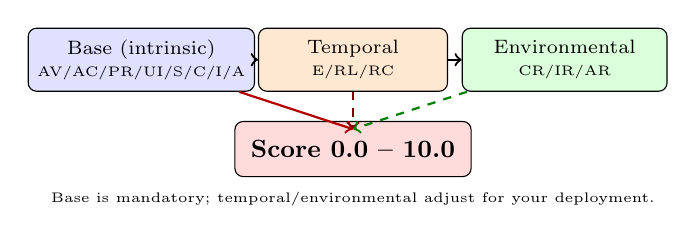
\begin{tikzpicture}[scale=0.84,every node/.style={font=\scriptsize}]
  \node[draw,fill=blue!12,rounded corners=3pt,minimum width=2.6cm,minimum height=0.8cm,align=center] (base) at (-3.2,0) {Base (intrinsic)\\ \tiny AV/AC/PR/UI/S/C/I/A};
  \node[draw,fill=orange!18,rounded corners=3pt,minimum width=2.4cm,minimum height=0.8cm,align=center] (temp) at (0,0) {Temporal\\ \tiny E/RL/RC};
  \node[draw,fill=green!14,rounded corners=3pt,minimum width=2.6cm,minimum height=0.8cm,align=center] (env) at (3.2,0) {Environmental\\ \tiny CR/IR/AR};
  \draw[->,thick] (base) -- (temp); \draw[->,thick] (temp) -- (env);
  \node[draw,fill=red!14,rounded corners=3pt,minimum width=3.0cm,minimum height=0.7cm,align=center,font=\small\bfseries] at (0,-1.35) {Score 0.0 -- 10.0};
  \draw[->,thick,red!70!black] (base) -- (0,-1.05); \draw[->,thick,red!50!black,dashed] (temp) -- (0,-1.05); \draw[->,thick,green!50!black,dashed] (env) -- (0,-1.05);
  \node[font=\tiny,align=center] at (0,-2.1) {Base is mandatory; temporal/environmental adjust for your deployment.};
\end{tikzpicture}
\caption{CVSS groups. Base metrics describe the bug itself; temporal metrics describe exploit maturity and remediation; environmental metrics adjust for the asset's business value.}
\label{fig:cvss-groups}
\end{figure}

\begin{lstlisting}[language=Python]
# CVSS vector intuition (illustrative; real scoring uses FIRST calculator)
vector = "CVSS:3.1/AV:N/AC:L/PR:N/UI:N/S:U/C:H/I:H/A:H"
# Network, Low complexity, No privileges, No user interaction, High impact on C/I/A
# => Critical (9.8) : unauthenticated remote code execution over the network
# Contrast: AV:P/AC:H/PR:H/UI:R/C:L  => Low (1.x) : needs physical access + admin + user click
def severity(score):
    if score >= 9.0: return "Critical"
    if score >= 7.0: return "High"
    if score >= 4.0: return "Medium"
    if score > 0: return "Low"
    return "None"
print(severity(9.8))  # Critical
\end{lstlisting}

Use CVSS to prioritise, not to decide alone: a Medium on the payment service may outrank a High on an internal tool. Pair the score with asset value (environmental metrics) and exploit availability (is there a public PoC? is it wormable?). Track mean-time-to-patch by severity band as an engineering KPI.

 a Medium on the payment service may outrank a High on an internal tool. Pair the score with asset value (environmental metrics) and exploit availability.

\begin{figure}[h]\centering
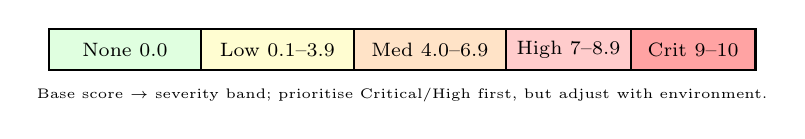
\begin{tikzpicture}[scale=0.88,every node/.style={font=\scriptsize}]
  \draw[thick,fill=green!12] (0,0) rectangle (2.2,0.6) node[midway] {None 0.0};
  \draw[thick,fill=yellow!18] (2.2,0) rectangle (4.4,0.6) node[midway] {Low 0.1--3.9};
  \draw[thick,fill=orange!22] (4.4,0) rectangle (6.6,0.6) node[midway] {Med 4.0--6.9};
  \draw[thick,fill=red!20] (6.6,0) rectangle (8.4,0.6) node[midway] {High 7--8.9};
  \draw[thick,fill=red!36] (8.4,0) rectangle (10.2,0.6) node[midway] {Crit 9--10};
  \node[font=\tiny,align=center] at (5.1,-0.35) {Base score $\to$ severity band; prioritise Critical/High first, but adjust with environment.};
\end{tikzpicture}
\caption{CVSS severity bands. The numeric score maps to a band; engineering priority also weighs asset exposure and exploit-in-the-wild status.}
\label{fig:cvss-bands}
\end{figure}

% ============================================================
\section{Metrics and Continuous Improvement}
\label{sec:metrics}
What gets measured gets fixed. Useful SDL metrics: time to fix by CVSS band, \% of features with a threat-model artefact, fuzz coverage and corpus size trends, SAST true-positive rate, and repeat-bug rate (same root cause twice). Review quarterly; a repeat bug means the SDL change from the last post-mortem did not land.

% ============================================================
\section{Incident Response}
\label{sec:ir}
No lifecycle ends at deployment. NIST SP 800-61 defines six phases: Prepare, Detect, Contain, Eradicate, Recover, Lessons Learned. The goal is to shrink dwell time and prevent recurrence, not to assign blame.

\begin{description}[leftmargin=1.2em,itemsep=0.35em]
    \item[Prepare] Playbooks, logging, backups, and tabletop exercises. If you have not rehearsed (tabletop exercise where the team walks a scenario like ``secret leaked on GitHub''), you are not prepared. Rehearsals surface missing logs, unclear ownership, and slow revocation before a real incident does.

, you are not prepared.
    \item[Detect \& analyse] Alerts from monitoring, SAST/DAST, and user reports; triage with CVSS + asset value; preserve evidence.
    \item[Contain] Short-term (isolate host, block IP, revoke token) then long-term (patch, firewall rule, feature flag).
    \item[Eradicate \& recover] Remove persistence, patch the root cause, restore from known-good, verify with tests.
    \item[Lessons learned] Blameless post-mortem, update SDL artefacts (requirements, threat model, tests) so the bug class cannot return.
\end{description}

\begin{lstlisting}[language=Python]
# Minimal post-mortem template (store with the fix)
post_mortem = {
    "title": "Export CSV leaked cross-tenant data",
    "severity": "High (CVSS 7.5) -- AV:N/AC:L/PR:L/UI:N/S:U/C:H/I:N/A:N",
    "root_cause": "Missing tenant_id check in export query; taint source reached sink without sanitizer",
    "fix": "Add tenant guard + add CodeQL taint rule + regression test with two tenants",
    "action_items": ["taint rule landed", "fuzz export", "threat model updated"],
    "lessons": "SDL design review now required for any cross-tenant feature"
}
\end{lstlisting}

\begin{remark}[Supply-chain SDL]
Dependencies are part of your attack surface. Pin versions, vet updates, require Sigstore signatures and SLSA provenance, and run SCA (software composition analysis) in CI to flag known CVEs in transitive deps. An SDL that ignores the supply chain secures the house while leaving the windows open.

\end{remark}

\begin{remark}[Culture]
Response quality is cultural: blameless post-mortems, no heroics, and a bias to fix the class, not just the instance. Every incident that does not update the SDL is a bug class waiting to fire again.
\end{remark}


\begin{remark}[Threat model debt]
Like technical debt, skipped threat models accumulate. Track the number of features shipped without a model and the time from model to mitigation; both trending down is a sign the SDL is real, not just a document. Auditors and customers increasingly ask for these artefacts.

\end{remark}


\begin{example}[CVSS in prioritisation]
Two bugs: (A) CVSS 9.8 RCE on an internal tool behind VPN (environmental: CR:L), (B) CVSS 6.5 XSS on the payment page (CR:H, exploit in the wild). Environmental scoring plus exploit maturity correctly ranks B above A for the next sprint. The raw base score alone would mislead.
\end{example}

\begin{remark}[Security champions]
Embed a security champion in each feature team: not a gatekeeper but a reviewer who can draw the DFD, run the taint query, and call the IR tabletop. Champions scale the SDL without centralising it into a bottleneck.
\end{remark}


\begin{remark}[Bug bars]
A bug bar defines the severity threshold that blocks release (e.g., ``no Critical/High, Medium with exploit in the wild must be fixed or risk-accepted by security''). It makes the SDL's exit criteria explicit and prevents last-minute debates about whether a bug can ship.
\end{remark}

% ============================================================
\section{Exercises}
\label{sec:ch08-exercises}
\begin{enumerate}[label=E8.\arabic*, leftmargin=*, itemsep=0.6em]
    \item \textbf{SDL mapping.} Your team adds ``sign in with OAuth.'' For each SDL phase list one concrete activity (e.g., Requirements: abuse case ``attacker links victim's account''). Which phase catches the cheapest fix if you skip it?
    \item \textbf{CVSS scoring.} Score: unauthenticated network RCE that gives full C/I/A, no user interaction. Choose AV/AC/PR/UI/S and estimate the base score band. How would S=C change the score compared with S=U?
    \item \textbf{Threat model delta.} A new admin bulk-import via CSV is proposed (upload $\to$ parse $\to$ DB). Draw the DFD delta, STRIDE it, and propose three mitigations. Which residual risk would you accept vs.\ must-fix before ship?
    \item \textbf{IR tabletop.} A secret key is found in a public GitHub repo. Walk the six IR phases, listing the first three commands or tickets you would create in each of Contain, Eradicate and Lessons Learned.
    \item \textbf{Post-mortem as code.} Write a one-page post-mortem for a reflected XSS that was deployed behind a weak CSP (\texttt{script-src 'unsafe-inline'}). Include root cause, CVSS, fix (encoding + CSP nonce), and the SDL change that prevents the class.
\end{enumerate}

\section*{Chapter Notes}
SDL from Howard \& Lipner, \emph{The Security Development Lifecycle} (Microsoft, 2006); modern variants include BSIMM and Google's SSDL. CVSS v3.1 is FIRST (2019); v4.0 (2023) adds granularity. Incident response is NIST SP 800-61; post-mortem culture from Allspaw and the SRE playbook; threat-model integration from Shostack.

% End of Chapter 8
